\documentclass[11pt,twoside,a4paper]{article}

\usepackage{hyperref}
\usepackage{graphicx}
\usepackage{wrapfig}
\usepackage{subcaption}
\usepackage{chngpage}
\usepackage{amsmath}

\begin{document}
%
\includegraphics[width = 40mm]{polito.png}
\title{Machine Learning and Artificial Intelligence Homework 2}
\author{Matteo Borghesi \textit{(s268199)}}
\maketitle

\section{Introduction}
In the course of this report we are going to train a convolutional neural network for an image classification task. In particular, our goal is to build a deep learning model through the Python language to assign correctly previously unseen images to one of 101 categories.\newline
In order to do that we use the Caltech dataset, which consists of 9146 images, divided unevenly across the categories (each category can have from 40 to 800 images); the size of the images is roughly 300 x 200 pixels. Fig.~\ref{fig:caltech} shows as an example two images taken from this dataset, labeled respectibely as \textit{snoopy} and \textit{cannon}.

\begin{figure}[!b]
    \centering
    \begin{subfigure}{0.35\textwidth}
	
\includegraphics[width=\linewidth]{snoopy.jpg}
        \caption{}
    \end{subfigure}
    \begin{subfigure}{0.35\textwidth}
	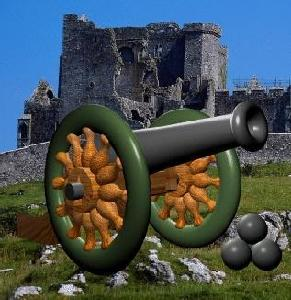
\includegraphics[width=\linewidth]{cannon.jpg}
        \caption{}
    \end{subfigure}
    \caption{Sample images from the Caltech dataset}
    \label{fig:caltech}
\end{figure}

The network architecture is given by AlexNet, which has been one of the most widely used networks since it succeeded at the ImageNet Visual Recognition Challenge in 2012. AlexNet consists of 8 main layers, divided in two segments: the first five are convolutional layers, some of which are followed by max-pooling layers, while the last ones are fully-connected. The last layer outputs a 1000-dimensional vector, which contains the score of each class. Inside the neurons a non-saturating ReLU activation function is employed, which solves the problem of 'killing' the gradients that is typical of the sigmoind and tanh functions.



\section{Data preparation}
\subsection{Caltech class}
As usual, to build a machine learning model it's necessary fist to partition reasonably the data set, so that all three stages of training, validation and testing have their own material to work on. In this case the splitting between training end testing data is provided upfront by means of two text files, named \textit{train.txt} and \textit{test.txt}, that indicate which image files belong to each bucket.\newline
In order to load the data set in the Python environment, we define a subclass \textit{Caltech} of VisionDataset, so that we can reuse some of its functionalities, like other PyTorch classes such as DatasetFolder and ImageFolder do. However, differently from these two examples we prefer to keep our PIL images in the main memory rather than always having to retrieve them from the file system at access time.\newline
Therefore, we customize the initialization functions, called in the constructor method, giving them the logic to retrieve the images as dictated in the text files and to store the images directly in the Caltech object. Furthermore, the initialization function perform the desired transformation on the input images, e.g. normalizing them and adapting their size to the input required by AlexNet, which amounts to 224x224 pixels. This design also provides for scalability in case of data augmentation, as we will see in sec.~\ref{dataAugmen}.\newline
At the end of this phase, we will have two Caltech objects, containing respectively 5784 samples (for the training phase) and 2893 samples (for the test phase).

\subsection{Validation set}
As a next step, the training set has to be split between the actual training samples, that will be used to train the neural network, and the validation set, which serves to evaluate the performance of the network after each epoch in order to get a good bias-variance tradeoff. Our goal is to use roughly \( \frac{2}{3} \) of the items for training and the rest for validation.\newline
Since the samples are already sorted according to their label inside the Caltech object, it suffices to walk once through the training set and move every third item to the validation set, which will be represented by a further Caltech object. In case the number of samples of one category is not divisible by 3, we prefer to include one of the remaining items (which are either one or two) in the validation set, in order to have a better balance between the two sets. According to this algorithm, the actual training set will contain 3824 items, while the validation set will have 1960 (which corresponds 33,88\% of the samples).

\section{Network setup}
\label{netSetup}
At the beginning, we train the network for 30 epochs basing on the Cross Entropy loss function. This function is defined as the negative logarithm of the softmax function, computed on all the class scores. In other words, we use the softmax to normalize the scores output in the forward pass, and use the negative logarithm in order to make it easy to perform the minimization.\newline
The gradients are updated at each steap according to the Stochastic Gradient Descent (SGD) with momentum, with an initial learning rate of $10^{-3}$. The learning rate is subject to a decay by a factor 0.1 every 20 epochs. Each step is executed on a batch of 256 items, which means it takes 14 steps to complete an epoch.\newline
Finally, before starting the training we must adapt the structure of AlexNet to our concrete problem, which considers only 101 categories instead of the default value of 1000. Therefore we replace the last fully-connected layer in the network with another layer of the same kind, but this time with a 101-dimensional output.

\section{Model selection}
\label{modSel}
The goal of having a validation set is to be able to estimate the performance of the model at different stages of the training phase. In the case of deep learning, the parameters of the model change at every training step: therefore, the model selection consists in choosing a 'snapshot' of the network with parameters which are considered to be optimal. The quality of the model is assessed by means of the classification accuracy on the validation set.\newline
At the beginning, accuracy typically increases, as the model learns the key features about the dataset. However, after a while it can happen that the network specializes too much on the images in the training set and is not able to generalize to new images. The accuracy, differently than the loss function, captures the capability to generalize to new samples, so that we can have a model that is free from overfitting. \newline
In this regard, fig.~\ref{fig:modelSel} plots the loss function and the accuracy on the validation set as the training phase proceeds. The highest accuracy - which is 13.62\% - is reached after 25 epochs, therefore we use this number to train our final model and then test it on the test set, which results in a 14.44\% accuracy.

\begin{figure}[]
    \centering
    \begin{subfigure}{0.45\textwidth}
	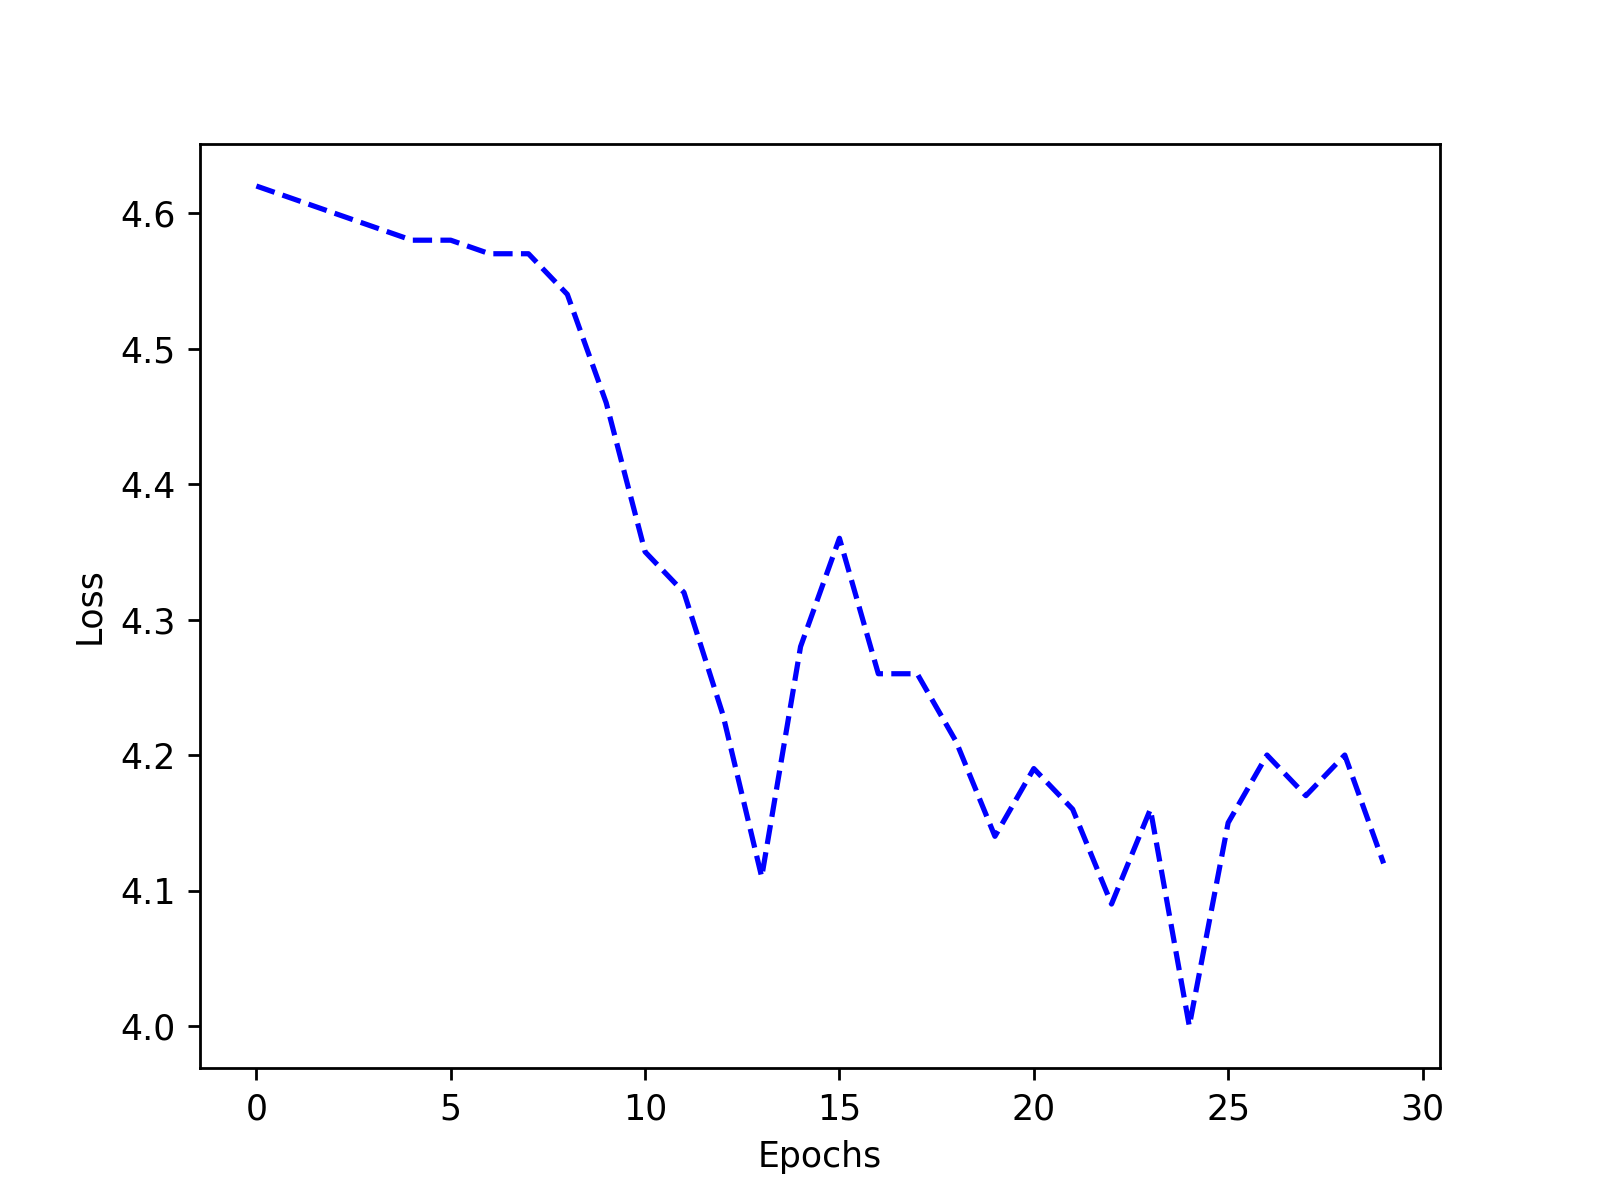
\includegraphics[width=\linewidth]{loss.png}
        \caption{}
    \end{subfigure}
    \begin{subfigure}{0.45\textwidth}
	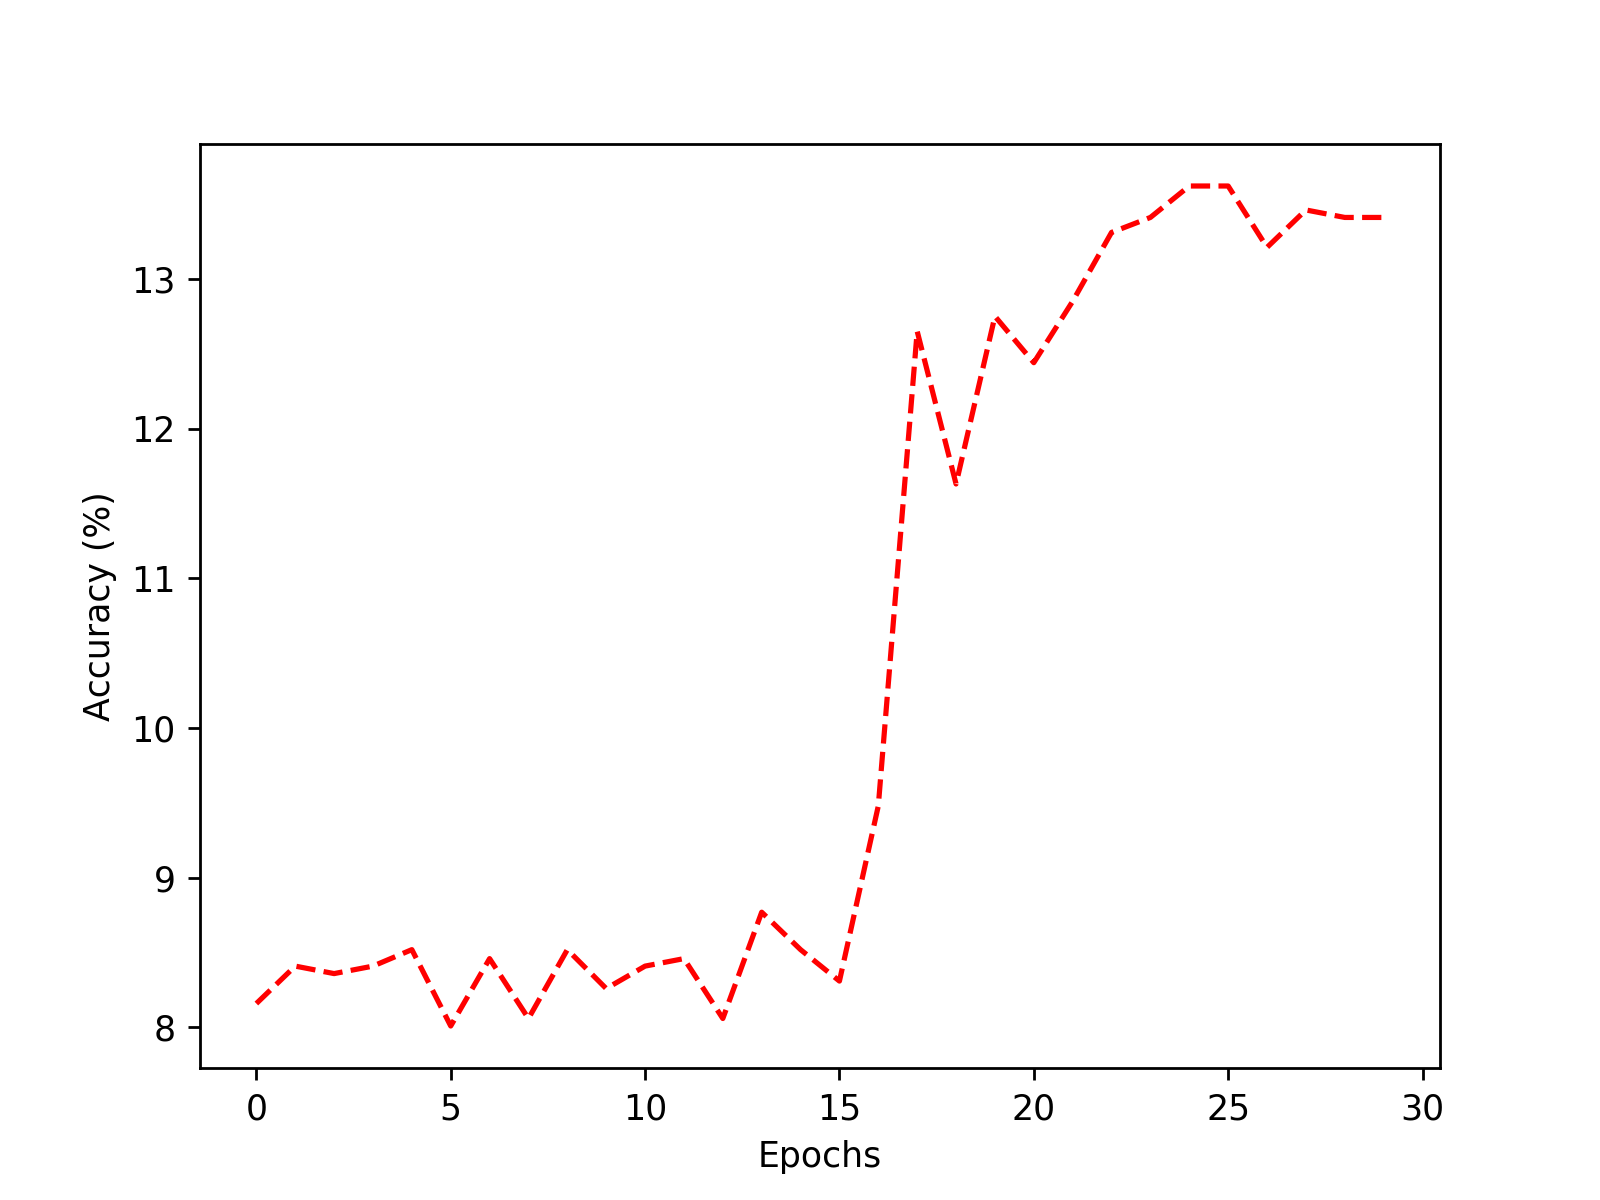
\includegraphics[width=\linewidth]{accuracy.png}
        \caption{}
    \end{subfigure}
    \caption{Loss (a) and validation accuracy (b) in the training phase}
    \label{fig:modelSel}
\end{figure}

\section{Hyperparameter tuning}
\label{sec:hyperparams}
Hyperparameters can have a major impact on the training phase. The default hyperparameters for our analysis have been presented in sec.~\ref{netSetup}, now we will try different configurations and see if we can improve in this way the results obtained in sec.~\ref{modSel}.\newline
As a first step, we change the algorithm used to update the parameters in the backward pass, using Nesterov's method instead of SGD. Furthermore, we increase the weight decay from $5\cdot10^{-3}$ to $10^{-2}$: this increases the impact of regularization on the loss function, encouraging simpler models.\newline
Secondly, we use the default hyperparameters but increase the step size to 30. In this way we stick with the initial learning rate throughout the training, discarding the decaying policy: this brings the model to converge faster, since the parameters are updated in the direction of the optimal values in bigger leaps. On the other side, the final result may be less accurate, since there can be a loss of precision in the vicinity of the optimum.\newline
Finally we do the opposite, i.e. we intensify the reduction of the learning rate by decreasing the step size to 10; furthermore, we set a more strict decaying factor - called \textit{gamma} - which becomes now 0.01.

Table~\ref{tab:hyperparams1} shows the result of this exploration in the hyperparameter space: using the Nesterov momentum together with a higher weight decay leads to quite poor results; a lower learning rate also does not perform better than the first model. On the contrary, we notice that a higher learning rate has a significantly better accuracy: this goes against our previous predictions, about a faster but worse convergence in case of a high learning rate.\newline
As a consequence, we might derive that the first model did not reach convergence at all, and that after 30 epochs the parameters were still halfway through their optimization. In this case, we should conclude that the decrease in the validation accuracy seen in fig.~\ref{fig:modelSel} was not due to overfitting, but to random noise, which would be reasonable in the light of the rather small variation observed. In order to prove this assumption, we modify another hyperparameter, namely the number of epochs, bringing it to 60. This way, if there were still range of optimization we should observe an improvement in the accuracy as the model is trained beyond the standard 30 epochs.\newline
As Table~\ref{tab:hyperparams1} shows, this is indeed the case, as we reach a considerably better accuracy than before: the highest score of 20.3\% is observed after 57 epochs, so that it would make sense to further enlarge the number of training epochs.

\begin{table}[]
  \begin{adjustwidth}{-.5in}{-.5in}
  \begin{center}
    \begin{tabular}{l | c | c}
       Set & Validation accuracy (\%) & Test accuracy (\%) \\
      \hline
	Default & 13.62 & 14.44\\
	Nesterov+weight decay & 10.3 & 10.6\\
	Learning rate (high) & 19.33 & 21.36\\
	Learning rate (low) & 11.83 & 12.65\\
	Epochs & 20.3 & 21.6\\
    \end{tabular}
    \caption{Comparison of different hyperparameter sets}
    \label{tab:hyperparams1}
  \end{center}
  \end{adjustwidth}
\end{table}

\section{Transfer learning}
\label{sec:transfer}

\begin{figure}[!b]
    \centering
    \begin{subfigure}{0.4\textwidth}
	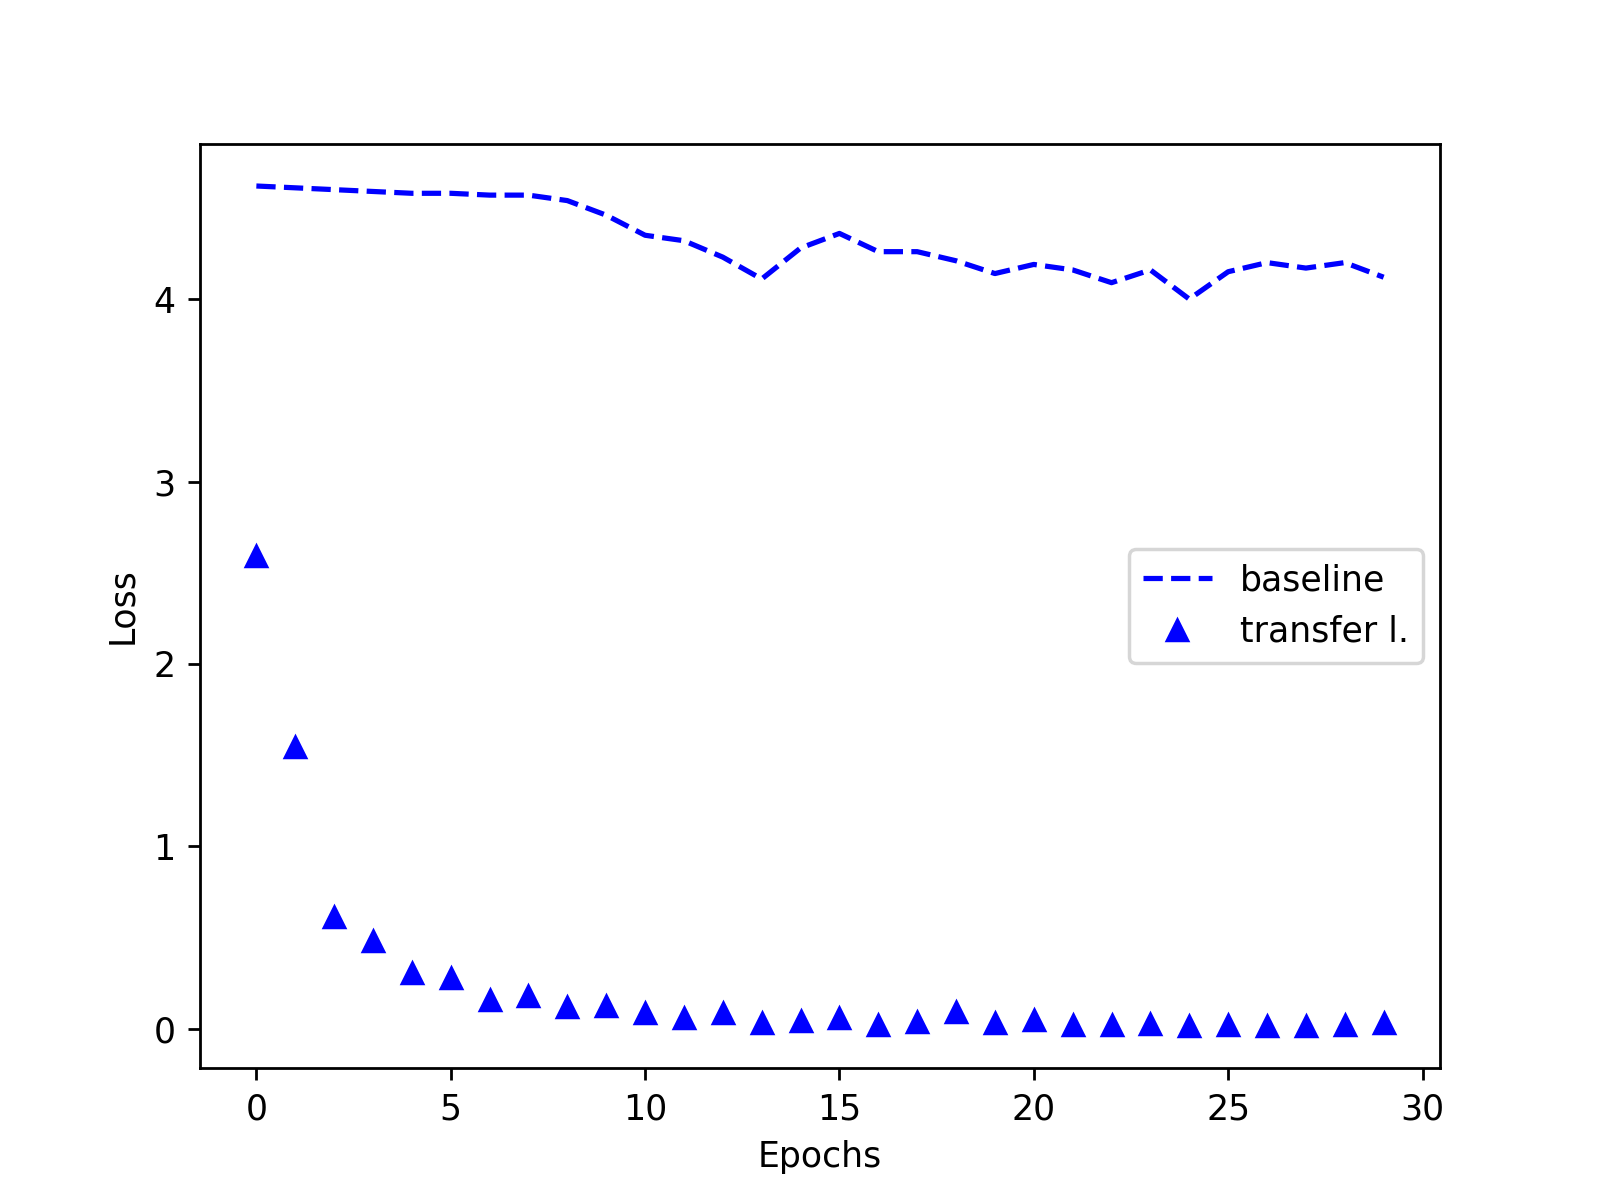
\includegraphics[width=\linewidth]{transfer_loss.png}
        \caption{}
    \end{subfigure}
    \begin{subfigure}{0.4\textwidth}
	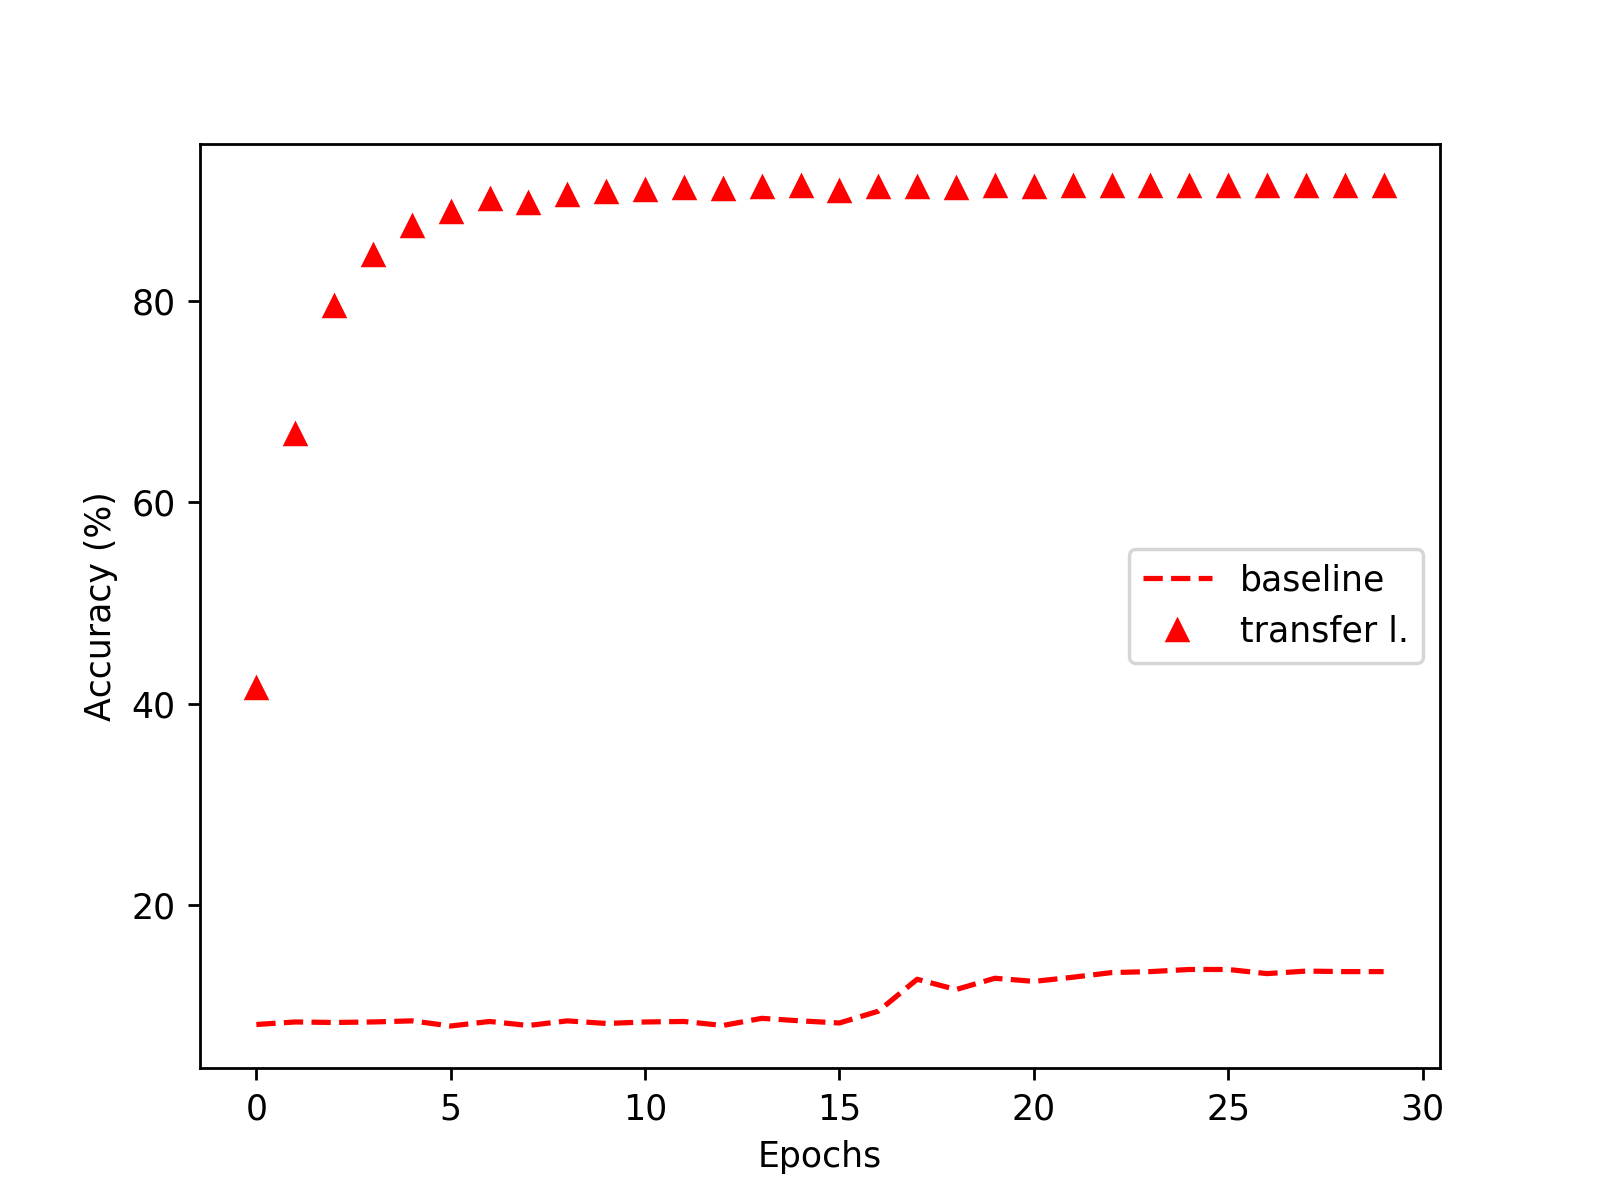
\includegraphics[width=\linewidth]{transfer_accuracy.png}
        \caption{}
    \end{subfigure}
    \caption{Loss (a) and validation accuracy (b) using transfer learning compared to the baseline from fig.~\ref{fig:modelSel}}
    \label{fig:transfer}
\end{figure}

Neural networks typically need huge amounts of data in order to be operationally effective, in this case for classification. This represents a considerable drawback in our setting, since the 3824 items in the training set are few compared to the needs of the network, as witnessed by the results sofar. In order to address this issue, it's possible to resort to a technique called transfer learning, which consists in exploiting the knowledge coming from a pretrained network and 'finetuning' it to the specific data we are interested in.\newline
Concretely, we use a version of the AlexNet trained on the ImageNet dataset, which contains objects from over 20.000 categories, including many of the ones used in the Caltech dataset. The pretrained AlexNet is directly available in the PyTorch library, hence we can easily include its benefits in the Python code used to perform the current analysis.

Clearly, since the starting parameters are now calibrated on the data in ImageNet we need to feed the Caltech images to the network as if they came from the same distribution as the other training data. Concretely, we normalize the input images with the mean and standard deviation from ImageNet, which are the vectors (0.485, 0.456, 0.406) and (0.229, 0.224, 0.224), whereby each value refers to one of the three RGB attibutes. Fig.~\ref{fig:transfer} shows the stunning performance achieved with transfer learning in comparison with the training done in sec.~\ref{modSel}: in particular, the validation accuracy is boosted from 13.62\% to as much as 91.37\%.\newline
Also here, we perform the train with the different hyperparameters presented in sec.~\ref{sec:hyperparams}. The results are shown in Table~\ref{tab:hyperparams2}: again, the best performance is obtained incrementing the number of training epochs.\newline

\begin{table}[!t]
  \begin{adjustwidth}{-.5in}{-.5in}
  \begin{center}
    \begin{tabular}{l | c | c}
       Set & Validation accuracy (\%) & Test accuracy (\%) \\
      \hline
	Default & 91.37 & 87.1\\
	Nesterov+weight decay & 91.37 & 86.62\\
	Learning rate (high) & 91.37 & 87.07\\
	Learning rate (low) & 91.22 & 86.27\\
	Epochs & 91.42 & 87.41\\
    \end{tabular}
    \caption{Comparison of different hyperparameter sets using transfer learning}
    \label{tab:hyperparams2}
  \end{center}
  \end{adjustwidth}
\end{table}

\begin{table}[!b]
  \begin{adjustwidth}{-.5in}{-.5in}
  \begin{center}
    \begin{tabular}{l | c | c}
       & Validation accuracy (\%) & Test accuracy (\%) \\
      \hline
	All layers & 91.42 & 87.41\\
	FC layers only & 91.32 & 87.52\\
	Convolutional layers only & 50.25 & 49.87\\
    \end{tabular}
    \caption{Results obtained training different parts of the network}
    \label{tab:freeze}
  \end{center}
  \end{adjustwidth}
\end{table}

Now that we have reached satisfactory results, we can think about accelerating the training phase, which can become a burden in certain contexts. In order to do that, it's possible to 'freeze' some part of the network, i.e. performing the training only on a subset of the layers. For this training phase, we choose the hyperparameter set that has had the best results in the last step, as summarized in Table~\ref{tab:hyperparams2}: the choice - in this case extending the train to 60 epochs - must be done according to the validation accuracy, since using test results for any kind of model configuration would tamper the scientificity of the result. To perform the analysis, we first freeze the convolutional layers (called \textit{features} in the PyTorch implementation) and train the fully connected part (the \textit{classifier}), then we do the opposite.\newline
The results are shown in Table~\ref{tab:freeze}: freezing the convolutional layers does not harm the precision of the model, since that part typically deals with generic features of the images, that can be extensively learned in the pretraining phase (done on ImageNet). Instead, freezing the fully-connected layers brings to poor performances, since those are in charge of the final classification according to the specific categories in the Caltech dataset. For the last part, we will freeze the first part of the network, in order to drop significantly the training time without loosing too much in accuracy.

\section{Data augmentation}
\label{dataAugmen}
As we have seen in sec.~\ref{sec:transfer}, the amount of data can play a fundamental role in the performance of a neural network. In this section we keep following this idea incrementing not only the data used to increment the network overall, as we did with transfer learning, but also the data used to finetune the network to the Caltech dataset. We do this by transforming the input images in such a way that they are still likely to belong to the original distribution, so that we can provide them to the network in addition to their original version.\newline
Actually, we have already transformed the images in the Caltech dataset all along by cropping the central 224x224 patch, in order to adapt the image size to the needs of the AlexNet. Therefore, a first way to perform data augmentation - as this technique is called - is to add images resulting from a random crop, instead of a central one. This can teach the network to recognize objects by seeing only a part of them, which can be useful at test time in case of occlusion.\newline
A second method to increase the size of data would be to include also an horizontally flipped version of the images, hence exchanging the left side with the right one. Vertical flipping, i.e. inverting the upper and the lower part, is less useful, since it's unlikely that we get a test time an elephant or a car turned upside down. Indeed, providing training data that are different from test data might bring the network to learn wrong features, with a decrease in the accuracy

Table~\ref{tab:freeze} shows the result of training with data augmentation. In order to mantain the same proportion between training and validation set, we have included the transformed images in the validation, although it is not necessary; on the contrary, the test set does not change.\newline
The test set In the first line we show the results obtained sofar, then in the next two lines we double the size of the training set, adding first the flipped images and then the randomly cropped images. In the end, we include both transformations in the dataset, which thus contains 11.472 images.

\begin{table}[!h]
  \begin{adjustwidth}{-.5in}{-.5in}
  \begin{center}
    \begin{tabular}{l | c | c}
       & Validation accuracy (\%) & Test accuracy (\%) \\
      \hline
	No augmentation & 91.32 & 87.52\\
	Flip & 97.88 & 87.57\\
	Random crop & 97.85 & 86.84\\
	Flip + random crop & 95.73 & 87.22\\
    \end{tabular}
    \caption{Results obtained training different parts of the network}
    \label{tab:freeze}
  \end{center}
  \end{adjustwidth}
\end{table}

\section{Other networks}
In this section, we explore two of the successors of AlexNet in the ImageNet competition: in particular, we use the VGGNet, that got the 2$^{nd}$ place in 2014 behind the GoogleNet, and the ResNet, which was the winner of the 2015 edition.\newline
The peculiarity of these networks, that allowed them to overcome the performance of Alexnet, is that they are significantly deeper: we use a 16-layer VGG (with respect to 8 in the AlexNet) and a 50-layer ResNet. As a consequence, those networks consume more memory, so that we have to reduce the batch size, i.e. the number of samples that pass through the network in the same step; however, this will bring to longer epochs, so that we can reduce the epochs without losing anything in the number of update iterations.

In the case of the VGGNet, we set the batch size to as little as 16 samples and we train the network for 10 epochs; when using the ResNet instead we have batches with 64 elements and 30 epochs. As for the other hyperparameters, we use the default values described in sec.\ref{sec:hyperparams}, since it would be unfair to compare the results with an already optimized version of the AlexNet; finally, all networks are pretrained on the ImageNet dataset.\newline
Table~\ref{tab:vggres} compares the results obtained in this phase: as in the ImageNet competition, ResNet has the best performance, with an impressing 95.92\% test accuracy, however the VGGNet too performs significantly better than the AlexNet, by over 6\%.

\begin{table}[!h]
  \begin{adjustwidth}{-.5in}{-.5in}
  \begin{center}
    \begin{tabular}{l | c | c}
       & Validation accuracy (\%) & Test accuracy (\%) \\
      \hline
	AlexNet & 91.37 & 87.1\\
	VGGNet & 97.95 & 93.77\\
	ResNet & 99.54 & 95.92\\
    \end{tabular}
    \caption{Comparison of three network architectures}
    \label{tab:vggres}
  \end{center}
  \end{adjustwidth}
\end{table}

\end{document}

